\chapter{Implementation}
\label{ch:implementation}
In this chapter we will cover how we implemented the different classes to run our workloads.
We will start with the graph and its components,
then move on to the different generators for the graph data,
the random graph components and the operation order.
Then we will show the workload class in section~\ref{ch:implementation:se:graphWorkload} and finally describe the database bindings in section~\ref{ch:implementation:se:graphDatabaseBindings}.

The code of our implementation can be seen on GitHub\footnote{\url{https://github.com/ChristianNavolskyi/YCSB}}.

\todo{Class diagram of my classes and introduce the upcoming explanation}

\begin{figure}
  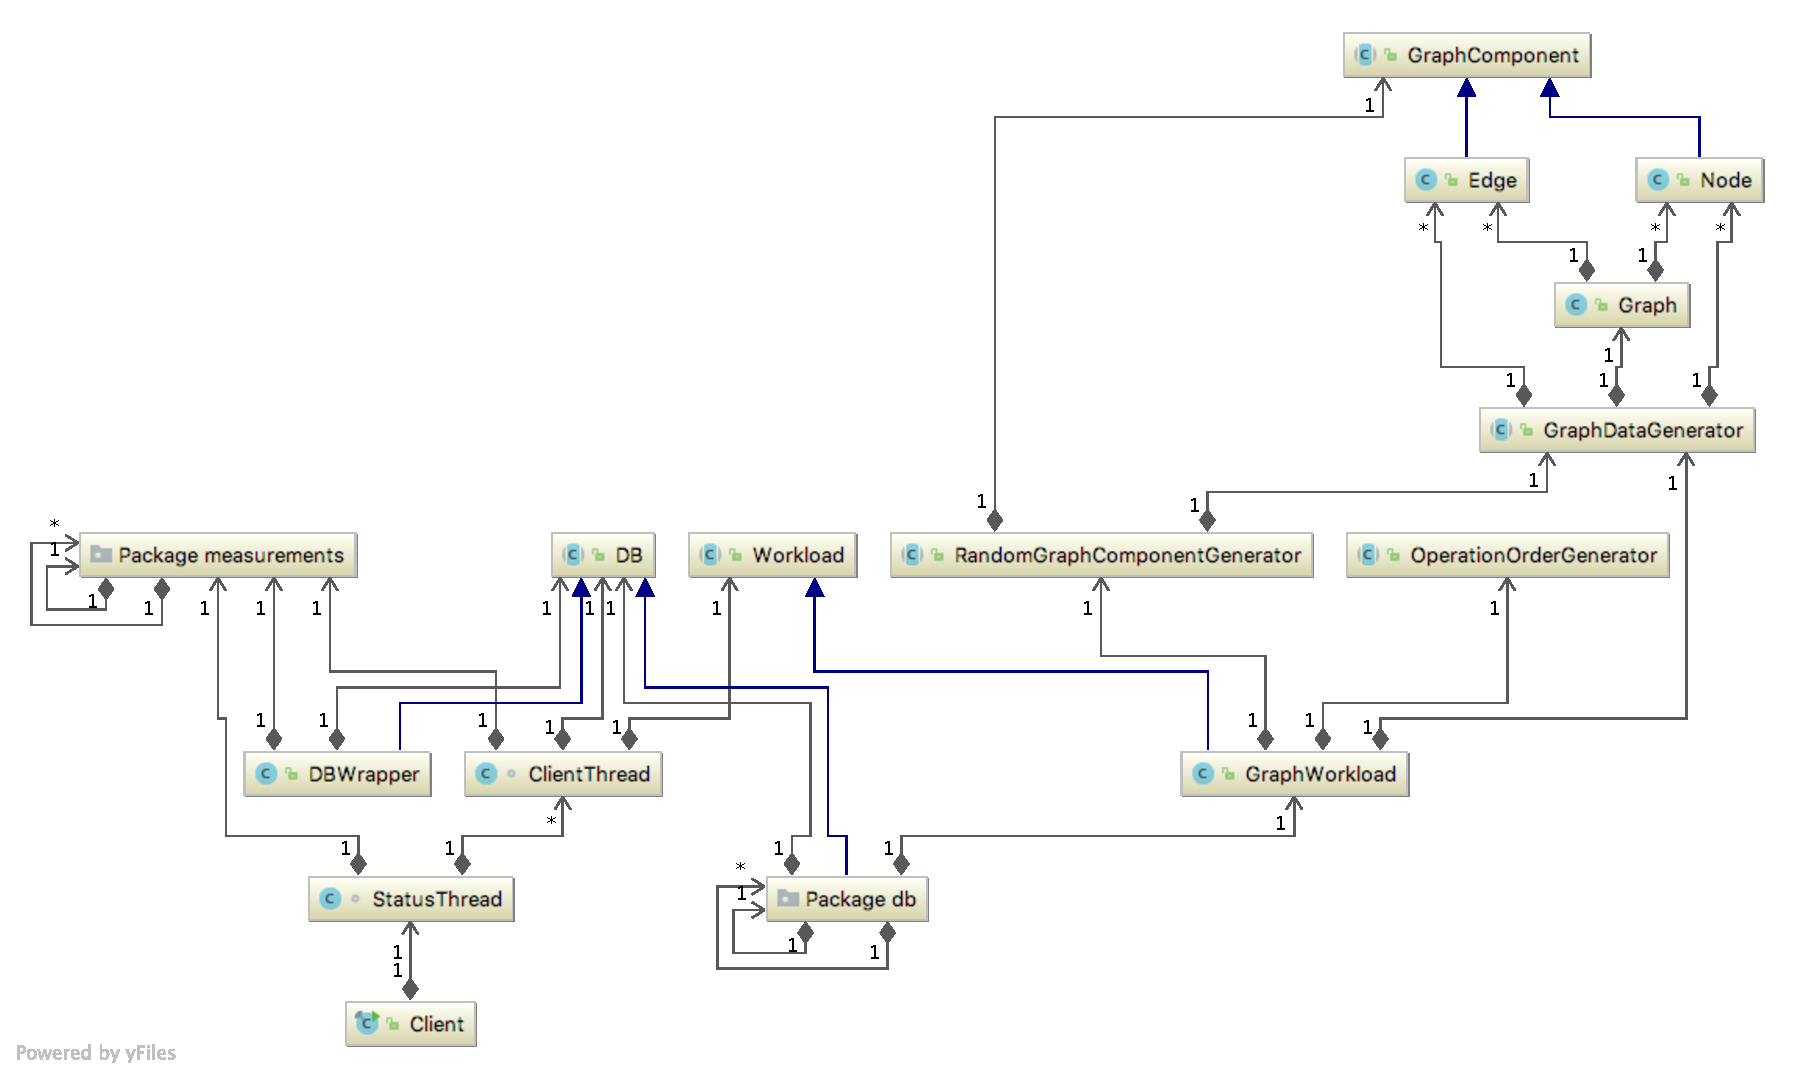
\includegraphics[width=\textwidth]{images/benchmarks/extendedYCSBWorkflow}
  \caption{Class diagram of YCSB with the classes we added to it. \todo{Reference AND Recreate with packages}}
  \label{fig:YCSBExtension}
\end{figure}

\section{Graph}
As mentioned in section~\ref{ch:background:se:graphs} a graph simply contains two lists,
one for nodes and one for edges.
This class is only a container for the two lists.

To extract some shared values of nodes and edges,
we added an abstract class $ GraphComponent $,
that holds the identifier and the label of the graph component.

\subsection{Node}
The $ Node $ class assigns the identifiers by counting the created nodes and incrementing the counter for every new node.
If the property value of a node is not set,
a call to $ Node::getHashMap $ will randomly fill the property with the amount of characters specified by the "node property size" option.

\subsection{Edge}
As the $ Node $ class the $ Edge $ class also uses a counter field to assign the correct identifier to each edge.

\section{Generator}
\label{ch:implementation:se:generator}
The general workflow of a generator was mentioned at the end of section~\ref{ch:design:se:summary}.
Because all three generators share that behaviour we created an abstract class $ StoringGenerator $\footnote{com.yahoo.ycsb.generator.StoringGenerator},
that extends the generic $ Generator<V> $\footnote{com.yahoo.ycsb.generator.Generator} class and adds methods to check if the files are present for recreation or not.

Every generator offers a $ create $ method,
in which it will check for present files and set up the correct implementation (recorder or recreator) for the $ GraphWorkload $\footnote{com.yahoo.ycsb.workloads.GraphWorkload} to use.
The generator classes are all abstract and use abstract methods to call the underlying implementation.
How this is useful will be described in the implementations of the different kinds of generators.

The abstract generator classes also contain the values needed for both implementation types (recorder and recreator),
to have them all in one place.

\subsection{Graph Data}
The $ nextValue $ call encapsulates the call to get the subgraph from the underlying implementation and also stores the returned identifiers of the created nodes and edges for the $ RandomGraphComponentGenerator $\footnote{com.yahoo.ycsb.generator.graph.randomcomponents.RandomGraphComponentGenerator},
that needs them to know which values it can return.

The $ Gson $\footnote{com.google.gson.Gson} used in both implementations of this abstract class is initialised here with the $ GraphAdapter $\footnote{com.yahoo.ycsb.generator.graph.GraphAdapter}.

Since there are two phases of the benchmark (see section~\ref{ch:analysis:se:ycsb}) the generator needs to know from which point it should move on with creation,
therefore if the current phase is the transaction phase,
it will call the the underlying implementation to create the amount of data that was created during the load phase,
to equalise the progress of the generator.
That is also important for the $ RandomGraphComponentGenerator $,
because the identifiers of the graph components created by the $ GraphDataGenerator $ are kept there for it to use them.

\subsection{Random Graph Component}
Calling $ nextValue $ on a $ RandomGraphComponentGenerator $ will invoke the implementing class to chose between a node and an edge and then chose a random graph component of that type.
A random node can also be picked directly,
that is needed for the $ GraphWorkload::update $ method,
since it only will use nodes.
\todo{maybe extend description}

\subsection{Operation Order}
Here the generator only holds common fields shared by the recorder and the recreator.
Besides that it offers the $ OperationOrderGenerator::create $ method,
which observes the present files and initialises the corresponding implementation for the $ Graph Workload $.

\section{Recorder}
\label{ch:implementation:se:recorder}
\todo{diagram to show methods used during nextValue call for the specific use of the classe.}
For every kind we have a creator that creates the initial values for the workload and stores them in a corresponding file for the recreator~\ref{ch:implementation:se:recreator}.

How the creation of the values is implemented in each generator is described in the following subsections~\ref{ch:implementation:se:graphDataRecorder}~to~\ref{ch:implementation:se:operationOrderRecorder}.

\subsection{Graph Data}
\todo{Code snippet of serialiser}
\label{ch:implementation:se:graphDataRecorder}
As shown in figure~\ref{fig:generalGeneratorWorkflow} when $ GraphDataGenerator::nextValue $\footnote{com.yahoo.ycsb.generator.graph.GraphDataGenerator} is called to create the next subgraph,
the $ GraphDataRecorder $ is called and creates the subgraph according to the diagram shown in figure~\ref{fig:dataCreation},
then serialises it and writes the string coming from serialisation into a file line by line.
\todo{maybe deepen the explanation of how the schema is represented in this class.}

The serialisation process is done in a $ GraphAdapter $ that implements both a $ JsonSerializer $\footnote{com.google.gson.JsonSerializer} and a $ JsonDeserialzer $\footnote{com.google.gson.JsonDeserialzer} with a $ Graph $ as the generic value.
Since a graph object contains two lists,
these lists are serialised into a JsonElement,
which will be retrieved as a string by calling $ Gson::toJson $.

\subsection{Random Graph Component}
To chose between a node and an edge a random number between zero and one will be picked ($ r \in \mathbb{N}_0 \wedge r \in [ 0, 1 ] $) and stored in a file.
To select a random graph component the $ GraphDataGenerator $ will be asked what the last id was and then a random value between zero and that number.
That value will also be stored in a file corresponding to the type of the graph component.

\subsection{Operation Order}
\label{ch:implementation:se:operationOrderRecorder}
The $ OperationOrderRecorder $\footnote{com.yahoo.ycsb.generator.operationorder.OperationOrderGenerator} receives a $ DiscreteGenerator $\footnote{com.yahoo.ycsb.generator.DiscreteGenerator},
which supplies the string values for the operations.
These values will be taken from the $ DiscreteGenerator $,
saved in a file and then returned to the caller.

\section{Recreator}
\label{ch:implementation:se:recreator}
To retrieve the values stored by the recorder classes described in section~\ref{ch:implementation:se:recorder} the upcoming recreators are needed.

\subsection{Graph Data}
\todo{Code snippet of deserialiser}
If the files for the data set are present the $ GraphDataRecreator $ will be called to return the next subgraph.
It does that by deserialising the next line with the $ Gson::fromJson $ method which uses the $ GraphAdapter $ described in subsection~\ref{ch:implementation:se:graphDataRecorder} together with a $ Type $\footnote{java.lang.reflect.Type}.

This classes uses a $ BufferedReader $\footnote{java.io.BufferedReader} to read the file line by line,
to avoid extensive memory usage.

\subsection{Random Graph Component}
\label{ch:implementation:se:randomGraphComponentRecreator}
At the beginning the files will be read and their values will be stored in three different $ Iterator<String> $\footnote{java.util.Iterator<E>} one for the type and the other two for the identifiers of the different kinds of graph components.

When a values is required the corresponding $ Iterator<String> $ returns the next value in the list and increments its pointer.

\subsection{Operation Order}
As the $ RandomGraphComponentRecreator $ from subsection~\ref{ch:implementation:se:randomGraphComponentRecreator},
this recreator reads the file directly during initialisation and stores the values in an $ Iterator<String> $.

Every time $ OperationOrderRecreator::nextValue $ is called the next line from the $ Iterator<String> $ is returned.

\section{Graph Workload}
\label{ch:implementation:se:graphWorkload}
\todo{Activity diagram of the workflow with graph data. Create Activity diagram with database from workload view.}
During initialisation the $ GraphWorkload $ creates the three generator mentioned in section~\ref{ch:implementation:se:generator},
by using the $ create $ method,
that way we will have the correct type of generator (recorder or recreator).
It also parses the parameters to get to know if "noEdges" should be used,
what the "property size" of a node should be,
how many fields should be scanned ("recordcount") and the "folder".
The "noEdges" parameter is needed to execute the operations on the correct available graph components.
"property size" is stored to be retrievable by the $ Node $ to know how much random value it should generate.
The "recordcount" option is needed for the $ scan $ operation.
Lastly the "folder" is used to create the folder for the dataset if it is not present and also pass it to the individual generators.

In the load phase the $ Client $\footnote{com.yahoo.ycsb.Client} calls $ GraphWorkload::doInsert $.
The $ GraphWorkload $ then retrieves a subgraph from the $ GraphDataGenerator $ by calling $ GraphDataGenerator::nextValue $,
separates it into its core graph components and calls the $ DB::insert $ method with each individual component to add them to the database one by one.

If the $ Client $ calls $ GraphWorkload::doTransaction $ the $ GraphWorkload $ will first get the operation to execute on the database by the $ OperationOrderGenerator $.
After that it has an implementation for every available database operation.

\textbf{doTransactionInsert} \newline
Works as in the $ doInsert $ method,
by taking a subgraph from the $ GraphDataGenerator $ and inserting its components one by one into the database.

\textbf{doTransactionRead}
Depending on the "noEdges" option the $ RandomGraphComponentGenerator $ will be asked for a graph component,
if the option is $ false $ or a node if the option is $ true $.
With the identifier of the graph component,
its type and its available fields the database is queried to look up those fields of the specified component.

\textbf{doTransactionScan} \newline
As in the $ doTransactionRead $ method a graph component is chosen from the $ RandomGraphComponentGenerator $ depending on the set "noEdges" option.
Then the necessary arguments from the graph component will be passed to the $ DB::scan $ method,
alongside the specified $ recordcount $.

\textbf{doTransactionUpdate} \newline
The $ update $ method is not used by our workloads,
but to make the $ GraphWorkload $ accessible to other workloads we implemented it as follows.
It also pick a random graph component and calls the $ DB::update $ method of the database.
If the graph component is a node,
its property value will be randomly assigned.

We did not implement the $ delete $ method of the database,
as we won't use it in our workloads and the $ CoreWorkload $ that we used as reference also did not use it.

\subsection{DBWrapper}
During implementation we noticed,
that the $ DBWrapper $\footnote{com.yahoo.ycsb.DBWrapper},
which measures the time of each operations on the database,
could not distinguish between nodes being inserted or edges.
Therefore we additionally adding a measurement that includes the table name in the measurement name,
because the database will get the information about the type of the graph component being used by the $ table $ parameter,
we can use it here to measure the nodes and edges separately.

\subsection{Parameters}
This subsection covers the naming of the parameters in the code.

\begin{table}[h!]
  \begin{minipage}{\textwidth}
    \begin{tabularx}{\textwidth}{ | X | X | }
      \hline
      Our name & Name in the code \\ \hline \hline
      folder & datasetdirectory \\ \hline
      products per order & productsperorder \\ \hline
      components per product & componentsperproduct \\ \hline
      test parameter count & testparametercount \\ \hline
      recordcount & maxscanlength \\ \hline
      no edges & onlynodes \\ \hline
      node property size & fieldlength \\ \hline
    \end{tabularx}
  \end{minipage}
  \caption{This table shows by which name the parameters can be found in the YCSB project.}
  \label{tab:parameterMapping}
\end{table}

The $ dbFolder $ option is different for each database and will be mentioned in the corresponding binding subsection.
The same goes for the $ useIndex $ option.

\section{Graph Database Bindings}
\label{ch:implementation:se:graphDatabaseBindings}
\todo{Code snippets for inserting node/edge and retrieving node/edge}
\note{Highlight the mapping of data and other specialities}
In this section we will describe the different binding implementations, their specialities and how they implemented the different operations mentioned in section~\ref{ch:design:se:bindings}.
Table~\ref{tab:bindingParameterMapping} shows the options for the different databases.

\begin{table}
  \begin{minipage}{\textwidth}
    \begin{tabularx}{\textwidth}{ | X | X | X | }
      \hline
      Database & Folder option & Index option \\ \hline \hline
      Apache Jena & outputdirectory & - \\ \hline
      Neo4j & neo4j.path & neo4j.index \\ \hline
      OrientDB & orientdb.url & orientdb.index \\ \hline
      Sparksee & sparksee.path & sparksee.index \\ \hline
    \end{tabularx}
  \end{minipage}
  \caption{Parameter names of the different databases for the database folder and the index option}
  \label{tab:bindingParameterMapping}
\end{table}

\subsection{Apache Jena}
To modify the database with Jena we need to start a transaction and specify if it is a read or a write transaction.
After that we retrieve the model of the database to work on the data.
When we are done with our operation we need to commit or abort the transaction,
similar to a relational database.

\textbf{creating a node} \newline
A node is created by calling $ Model::createResource $\footnote{org.apache.jena.rdf.model.Model} with the $ key $ as an $ AnonId $\footnote{org.apache.jena.rdf.model.AnonId}.

\textbf{creating an edge} \newline
To create an edge we use the $ Model::createProperty $ method with the $ key $ as the argument.
To connect the edge with their start and end node,
we have to add this triple to the model by calling $ Model::add $ with the start node,
the edge and the end node.

\textbf{adding properties to a node} \newline
Properties are mapped as statements in Jena and to create those we use the $ Model::createStatement $ method that takes the node, the key for the property and the property value as arguments.
After all statements are created we add them to the model with $ Model::add $ and the list of statements as the argument.

\textbf{adding properties to an edge} \newline
To add the properties to an edge,
which is a $ Property $\footnote{org.apache.jena.rdf.model.Property} in Jena,
we use the $ Property::addProperty $ method on the edge with the key of the property and the value of it as arguments.

\textbf{getting a node by its identifier} \newline
Retrieving a node is done by creating a resource with the same identifier,
Jena will look up their database if one already exists and the returned node will be equal to an existing one.

\textbf{getting an edge by its identifier} \newline
Similar to retrieving a node from the database we create a property with the key,
that returns a existing edge if one is present with the key.

\textbf{getting the values of a node} \newline
To get the values associated with a node,
we create a $ SimpleSelector $\footnote{org.apache.jena.rdf.model.SimpleSelector},
which acts like a query on the database.
We supply it the node and the key of the value and leaf the object of the query empty,
so it look the matching values up.

\textbf{getting the values of an edge} \newline
The values of an edge are fetched the same way.

\textbf{getting the outgoing edges of a node} \newline
To get these edges we list the properties of the node,
which are represented as edges.

\textbf{getting the start node of an edge} \newline
To do this,
we take the start property of the edge and look up that node on the dataset.

\textbf{removing a node} \newline
Removing a node is done by calling $ Model::removeAll $ twice,
once with the node as the subject and once with the node as the object of the statement.
That will remove all statements associated with that node,
which will finally remove the node from the database.

\textbf{removing an edge} \newline
Here we also call $ Model::removeAll $ but the with edge as the predicate of the statement.

\subsection{Neo4j}
If an $ Index $\footnote{org.neo4j.graphdb.index.Index<T extends PropertyContainer>} should be used we create two of them,
one for the $ Node $s\footnote{org.neo4j.graphdb.Node} and one for the $ Relationship $s\footnote{org.neo4j.graphdb.Relationship} (edges).
Neo4j also uses transaction,
but we don't need to specify their kind.
At the end of a transaction we call $ Transaction::success $\footnote{org.neo4j.graphdb.Transaction} to finish the transaction.

\textbf{creating a node} \newline
We create a node with the $ GraphDatabaseService::createNode $\footnote{org.neo4j.graphdb.GraphDatabaseService} method,
where we specify the $ key $ as the $ Label $\footnote{org.neo4j.graphdb.Label} of the node.
If an $ Index $ is used we then add the node to the index.
After that we specially add the identifier of the node as a property.

\textbf{creating an edge} \newline
For this we have to first create a $ RelationshipType $\footnote{org.neo4j.graphdb.RelationshipType} with the $ key $ as the name of the relationship.
Then we create a relationship from the start node to the end node by calling $ Node::createRelationshipTo $.
Finally we add the edge to the relationship $ Index $.

\textbf{adding properties to a node/an edge} \newline
Both $ Node $s and edges are $ PropertyContainer $s\footnote{org.neo4j.graphdb.PropertyContainer},
which support the setting of properties,
by calling $ PropertyContainer::setProperty $ with the key of the property and its value.

\textbf{getting a node by its identifier} \newline
When an $ Index $ is used a node can be looked up on it with $ Index::get $ and the key for the identifier and the identifier value.
Without an $ Index $ we call $ GraphDatabaseService::findNode $ with the label the key for the identifier and the identifier as arguments.

\textbf{getting an edge by its identifier} \newline
With an $ Index $ a $ Relationship $ can be found similar the a node.
Without it we have to iterate over all $ Relationship $s in the graph and check their type to match the $ key $.

\textbf{getting the values of a node/an edge} \newline
The $ ResourceContainer::getAllProperties $ method supplies all values set the node or edge.
We can simply parse the $ Map<String, Object> $\footnote{java.util.Map<K, V>} returned by it to the needed $ Map<String, ByteIterator> $.

\textbf{getting the outgoing edges of a node} \newline
$ Node $s offer a method to get their $ Relationships $ in a specified $ Direction $\footnote{org.neo4j.graphdb.Direction}.

\textbf{getting the start node of an edge} \newline
$ Relationship $s also offer a method to directly get their start node with $ Relationship::getStartNode $

\textbf{removing a node} \newline
To remove a $ Node $,
we look it up,
remove it from the node $ Index $ and then call $ Node::delete $ to remove it from the database.

\textbf{removing an edge} \newline
Here the procedure is similar,
except we remove it from the relationship $ Index $.

\subsection{OrientDB}
To create an index with OrientDB we call $ OrientGraph::createKeyIndex $\footnote{com.tinkerpop.blueprints.impls.orient.OrientGraph} with the key of the identifier and the class of graph components,
once with $ Vertex $\footnote{com.tinkerpop.blueprints.Vertex} and once with $ Edge $\footnote{com.tinkerpop.blueprints.Edge}.
As Neo4j OrientDB uses transactions to execute operations on the database,
which have to be closed when finished with the operation itself by calling $ OrientGraph::shutdown $.

\textbf{creating a node} \newline
To add a node,
we simpley call $ OrientGraph::addVertex $ with the $ key $ and the value map we want to put in.
Before we add the value map,
we have to transform the $ ByteIterator $\footnote{com.yahoo.ycsb.ByteIterator} values to $ String $s.

\textbf{creating an edge} \newline
An edge is created by calling $ OrientGraph::addEdge $ with the $ key $,
the start node,
the end node and a label,
which we will simply set to "Edge",
because the label of our values map will be set as a property.

\textbf{adding properties to a node} \newline
As mentioned in at "creating a node" the values for the properties are directly passed during creation.

\textbf{adding properties to an edge} \newline
We can add the values to an edge by calling $ OrientElement::setProperties $\footnote{com.tinkerpop.blueprints.impls.orient.OrientElement} with the map of string values.

\textbf{getting a node by its identifier} \newline
A node is looked up by $ OrientGraph::getVertices $ with the identifier key and the identifier value.

\textbf{getting an edge by its identifier} \newline
$ Edge $s can be retrieved similarly,
but by calling $ OrientGraph::getEdges $ with the according parameters.

\textbf{getting the values of a node/an edge} \newline
The properties of an $ OrientElement $ can be obtained by calling $ OrientElement::getProperties $.
The values of the returned map are then casted to $ ByteIterator $s.

\textbf{getting the outgoing edges of a node} \newline
The edges of a node can be gathered by calling $ OrientVertex::getEdges $ with the specified direction.

\textbf{getting the start node of an edge} \newline
The procedure is analogous to that of getting the outgoing edge of a node.
We call $ OrientEdge::getVertex $ with the specified direction.

\textbf{removing a node} \newline
The $ OrientGraph::removeVertex $ method can be used the the vertex to remove to delete the vertex from the database.

\textbf{removing an edge} \newline
As to remove a node,
the $ OrientGraph $ provides a method to remove an edge internally,
that means the connected nodes are not removed.

\subsection{Sparksee}
The index can be activated on certain attributes by $ Graph::indexAttribute $\footnote{com.sparsity.sparksee.gdb.Graph} with the attribute and the $ AttributeKind.Indexed $\footnote{com.sparsity.sparksee.gdb.AttributeKind} as its arguments.
Sparksee uses $ Session $s\footnote{com.sparsity.sparksee.gdb.Session} as transaction,
these are also closed at the end of the transaction.

\textbf{creating a node} \newline
To create a node we first are creating a type for the node,
which is the same for all nodes.
Then we call $ Graph::newNode $ and set a identifier attribute to store the $ key $ in the node.

\textbf{creating an edge} \newline
Here we are also first looking up the two corresponding nodes and then we create an edge type,
that is also the same for all edges.
Then we create an edge by calling $ Graph::newEdge $ with the type,
the start and the end node.
Lastly the identifier for the edge is set as an attribute.

\textbf{adding properties to a node/an edge} \newline
To add attributes we have to create an attribute in the database with the name of the property.
Then we call $ Graph::setAttribute $ with that attribute and its value.

\textbf{getting a node/an edge by its identifier} \newline
Retrieving a graph component works by creating a $ Value $\footnote{com.sparsity.sparksee.gdb.Value} with the key of the component,
which is then passed to the $ Graph::findObject $ method with the attribute specifying a node or an edge.

\textbf{getting the values of a node/an edge} \newline
The attributes of a graph component are obtained by calling $ Graph::getAttributes $,
which hands us an $ AttributeList $\footnote{com.sparsity.sparksee.gdb.AttributeList} that is then looked up for the attributes we want to get.

\textbf{getting the outgoing edges of a node} \newline
To get the edges connected to a node,
we call $ Graph::neighbors $ with the node, the type of edge and the direction.

\textbf{getting the start node of an edge} \newline
The $ EdgeData::getHead $ method serves us that node.

\textbf{removing a node/an edge} \newline
To remove a graph component from the database we look the component up and then call $ Graph::drop $ on it,
to delete it from the database.
